% !TeX program = pdflatex
% ---------------------------------------------------------------------------
%  simTIM -- ARES 2026 conference talk. Build: make
%  Backup slides are a separate document: simTIM_ARES26_backup.tex
% ---------------------------------------------------------------------------
% Shared preamble for the talk and the backup deck.
% Fragment: \input from both, not compiled on its own.

\documentclass[aspectratio=169, 11pt]{beamer}

\usetheme{metropolis}
\metroset{numbering=fraction, progressbar=frametitle, block=fill}

% Presenter notes. `make notes` defines \notesversion and produces a second PDF
% with the speaker notes beside each slide; the normal build ignores them.
\ifdefined\notesversion
  \setbeameroption{show notes on second screen=right}
\fi

\usepackage[T1]{fontenc}
\usepackage[utf8]{inputenc}
\usepackage{graphicx}
\usepackage{tikz}
\usepackage{qrcode}
\usepackage{appendixnumberbeamer}
\usetikzlibrary{arrows.meta, positioning, shapes.geometric, calc, fit,
                backgrounds, patterns, decorations.pathreplacing}

\graphicspath{{figures/}{../Paper/figures/}{../Sources/}}

% --- palette: identical to the colours simTIM uses in its own plots ---------
\definecolor{atkRed}{HTML}{C7410F}      % attacker / damage
\definecolor{atkOrange}{HTML}{E8993A}   % user-level access
\definecolor{atkYellow}{HTML}{F2DC8C}   % visible
\definecolor{defBlue}{HTML}{1F77B4}     % defender / cost
\definecolor{gainGold}{HTML}{E8A33D}    % attacker gain
\definecolor{inkGrey}{HTML}{6B6B6B}
\definecolor{paleGrey}{HTML}{E9E9E9}

\setbeamercolor{frametitle}{bg=atkRed}
\setbeamercolor{progress bar}{fg=defBlue}
\setbeamercolor{alerted text}{fg=atkRed}

\newcommand{\atk}[1]{\textcolor{atkRed}{\textbf{#1}}}

% hyperref writes titles into PDF metadata; keep beamer macros out of them
\pdfstringdefDisableCommands{\def\translate#1{#1}}


% --- title -----------------------------------------------------------------


\title{simTIM}
\subtitle{A Temporal Cybersecurity Simulator}
% each affiliation sits directly under its author; metropolis puts \date last
\author{\texorpdfstring{%
  \begin{tabular}{@{}l@{\hskip 14mm}l@{}}
    Noah Niclas Behrisch & Zolt\'an \'Ad\'am Mann\\[1mm]
    {\footnotesize\color{inkGrey}University of Halle-Wittenberg} &
    {\footnotesize\color{inkGrey}University of M\"unster}
  \end{tabular}}%
  {Noah Niclas Behrisch, Zolt\'an \'Ad\'am Mann}}
\institute{}
\date{ARES 2026}

\begin{document}

% ===========================================================================
\maketitle

% ===========================================================================
\begin{frame}[plain]{Why model cybersecurity?}
\vfill
\centering
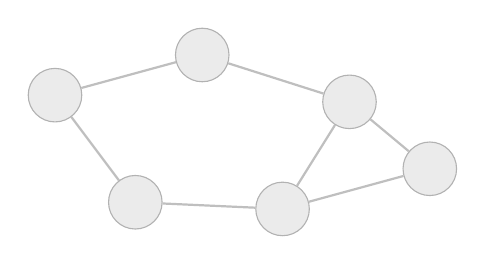
\begin{tikzpicture}[scale=0.85, transform shape,
   nd/.style={circle, draw=black!30, fill=black!8, minimum size=8mm}]
  \node[nd] (a) at (0,1.1) {};   \node[nd] (b) at (2.2,1.7) {};
  \node[nd] (c) at (4.4,1.0) {}; \node[nd] (d) at (1.2,-0.5) {};
  \node[nd] (e) at (3.4,-0.6) {};\node[nd] (f) at (5.6,0.0) {};
  \foreach \s/\t in {a/b, b/c, a/d, d/e, c/e, c/f, e/f}
     \draw[black!25, thick] (\s) -- (\t);
\end{tikzpicture}

\vspace{4mm}
{\large Which servers are vulnerable and need hardening?}\\[2.5mm]
{\large How should we change the network topology?}

\vspace{6mm}
{\Large Simulations provide \alert{what-if analysis}.}
\vfill
\note{%
\textbf{0:30--1:05.} Put them in the chair, do not read the questions verbatim.\\
Imagine you are a security analyst, or a network planner, at an organisation.
You have been given a budget and the task of improving security in the company
network. Which servers are particularly vulnerable and need hardening? How do
you optimise the topology?\\
What you would really like is what-if analysis --- and that is why there has
been so much research into modelling cybersecurity.%
}
\end{frame}

% ===========================================================================
\begin{frame}[plain]{TIM: three families of security models}
\vfill
\centering
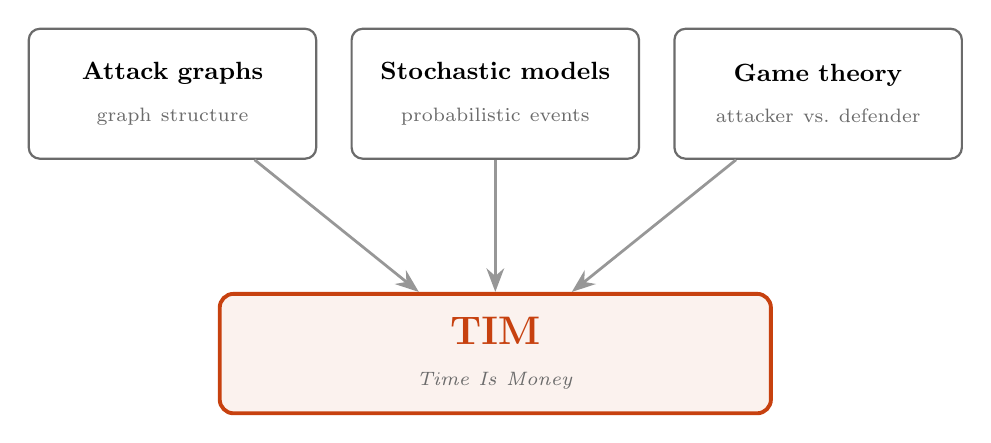
\begin{tikzpicture}[
   src/.style={rectangle, rounded corners=4pt, draw=inkGrey, thick, fill=white,
               text width=3.15cm, minimum height=1.65cm, inner sep=2.5mm,
               align=center},
   goal/.style={rectangle, rounded corners=5pt, draw=atkRed, line width=1.4pt,
                fill=atkRed!7, text width=6.4cm, minimum height=1.5cm,
                inner sep=3mm, align=center}]
\hyphenpenalty=10000 \exhyphenpenalty=10000

\node[src] (a) at (-4.1,1.55)
  {\textbf{\small Attack graphs}\\[1mm]
   {\scriptsize\color{inkGrey}graph structure}};
\node[src] (b) at (0,1.55)
  {\textbf{\small Stochastic models}\\[1mm]
   {\scriptsize\color{inkGrey}probabilistic events}};
\node[src] (c) at (4.1,1.55)
  {\textbf{\small Game theory}\\[1mm]
   {\scriptsize\color{inkGrey}attacker vs.\ defender}};

\node[goal] (t) at (0,-1.75)
  {\textcolor{atkRed}{\Large\bfseries TIM}\\[1mm]
   {\scriptsize\color{inkGrey}\emph{Time Is Money}}};

\foreach \s in {a,b,c}
  \draw[-{Stealth[length=3mm]}, inkGrey!70, line width=1pt] (\s) -- (t);
\end{tikzpicture}
\vfill
\note{%
\textbf{1:05--1:40.} Three sources, then the name.\\
One of these research efforts is the TIM meta-model, proposed by Zolt\'an. TIM
stands for ``Time Is Money''.\\
What makes it useful is that it combines three families of security models that
normally live apart: the graph structure of attack graphs, the probabilistic
events of stochastic models, and the attacker--defender framing of game theory.%
}
\end{frame}

% ===========================================================================
\begin{frame}[plain]{What TIM models}
\vfill
\begin{columns}[c,onlytextwidth]
  \begin{column}{0.58\textwidth}
    \centering
    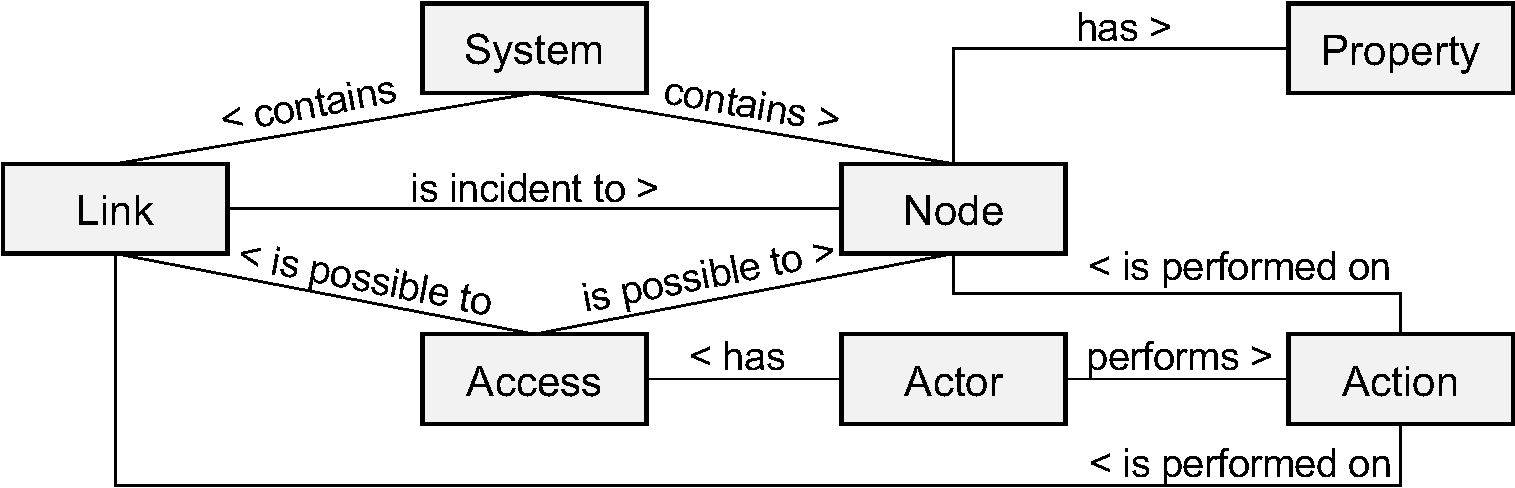
\includegraphics[width=\linewidth]{TIM_static_overview.pdf}
  \end{column}
  \begin{column}{0.40\textwidth}
    \small
    \textbf{Nodes} and \textbf{links}\\
    {\footnotesize\color{inkGrey}servers, routers, connections}\\[3.5mm]
    \textcolor{atkRed}{\textbf{Attackers}}: maximise gain\\[1.5mm]
    \textcolor{defBlue}{\textbf{Defenders}}: minimise damage\\[3.5mm]
    \textbf{Actions}\\[1mm]
    $a = (\varphi_a,\, \psi_a,\, c_a,\, d_a,\, p_a)$\\[1mm]
    {\scriptsize\color{inkGrey}precondition, postcondition,\\
     cost, duration, success probability}
  \end{column}
\end{columns}
\vfill
\note{%
\textbf{1:40--2:10.} Gesture at the diagram; do not read every box.\\
TIM models an organisation's IT assets. The network is composed of nodes and
links, which model servers, routers and the connections between them.\\
There are attackers, trying to make a monetary gain by exploiting the system,
and defenders, trying to minimise the damage to it. Both of these actors have a
host of actions they can employ to pursue their goal.\\
An action is a tuple: a precondition that has to hold for it to run, a
postcondition describing what it changes, a cost, a duration, and a success
probability. Do not read the symbols out --- name the five parts.%
}
\end{frame}

% ===========================================================================
\begin{frame}[plain]{Access levels}
% colours are simTIM's own (Okabe--Ito), so this doubles as a legend for the demo
\definecolor{accNone}{HTML}{0072B2}
\definecolor{accVis}{HTML}{F0E442}
\definecolor{accUser}{HTML}{E69F00}
\definecolor{accAdmin}{HTML}{D55E00}
\vfill
\centering
\begin{tikzpicture}[
   lv/.style={rectangle, rounded corners=3pt, draw=black!45, thick,
              minimum width=2.5cm, minimum height=0.95cm, font=\small\bfseries},
   lvcap/.style={font=\scriptsize, text=inkGrey, align=center}]
  \node[lv, fill=accNone, text=white]  (n) at (0,0)    {none};
  \node[lv, fill=accVis]   (v) at (3.0,0)  {visible};
  \node[lv, fill=accUser]  (u) at (6.0,0)  {user};
  \node[lv, fill=accAdmin, text=white] (a) at (9.0,0) {admin};

  \node[lvcap] at (0,-0.95)   {does not know\\ the node exists};
  \node[lvcap] at (3.0,-0.95) {knows it is there,\\ can reach it};
  \node[lvcap] at (6.0,-0.95) {user-level\\ access};
  \node[lvcap] at (9.0,-0.95) {full\\ control};

  \foreach \s/\t in {n/v, v/u, u/a}
    \draw[-{Stealth[length=2.5mm]}, black!45, thick] (\s) -- (\t);
\end{tikzpicture}

\vspace{3mm}
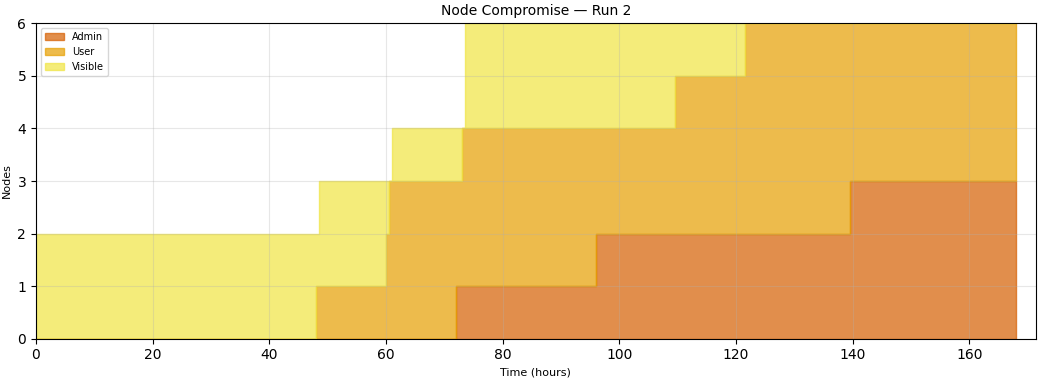
\includegraphics[width=0.80\textwidth]{access_timeline.png}
\vfill
\note{%
\textbf{2:10--2:35.} These are the same colours they will see in the demo ---
say so.\\
The access an actor has to a node is modelled in four levels: none, visible,
user and admin, and it is tracked separately for every actor. Gaining privileges
on a machine and moving laterally to the next one are both just changes of this
access level.\\
Point at the chart: that is one week of a real run, six nodes climbing from
visible, through user, to admin.\\
Then partial observability: the attacker starts out seeing only the nodes
exposed to the internet and has to discover the rest through their own actions.
The defender sees the whole network but does not automatically see the attacker,
because detection is probabilistic. Both sides act on incomplete information.%
}
\end{frame}

% ===========================================================================
\begin{frame}[plain]{Physical time}
\vfill
\centering
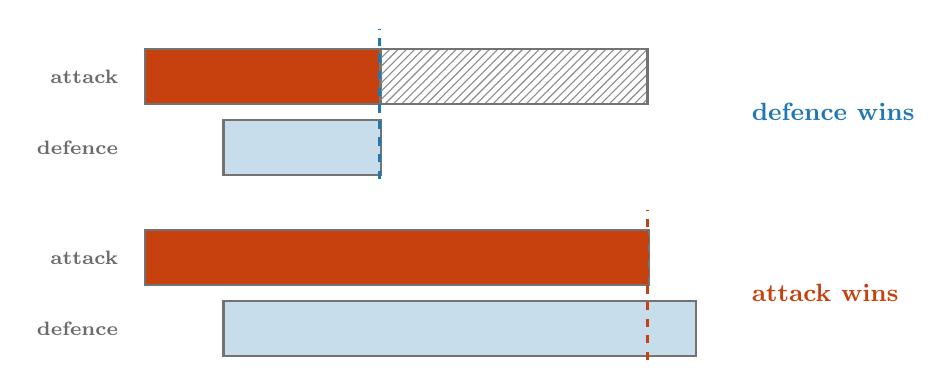
\begin{tikzpicture}[
   bar/.style={rectangle, draw=black!55, thick, minimum height=7mm,
               anchor=west, font=\scriptsize, inner sep=2pt},
   lbl/.style={font=\scriptsize\bfseries, anchor=east, text=inkGrey}]

\begin{scope}[yshift=2.3cm]
  \node[lbl] at (-0.2,0.95) {attack};
  \node[lbl] at (-0.2,0.05) {defence};
  \node[bar, fill=atkRed, text=white, minimum width=3.0cm] at (0,0.95) {};
  \fill[pattern=north east lines, pattern color=black!45, draw=black!55, thick]
       (3.0,0.6) rectangle (6.4,1.3);
  \node[bar, fill=defBlue!25, minimum width=2.0cm] at (1.0,0.05) {};
  \draw[defBlue, dashed, line width=1.2pt] (3.0,-0.35) -- (3.0,1.55);
  \node[anchor=west, font=\small\bfseries, text=defBlue] at (7.6,0.5)
       {defence wins};
\end{scope}

\begin{scope}
  \node[lbl] at (-0.2,0.95) {attack};
  \node[lbl] at (-0.2,0.05) {defence};
  \node[bar, fill=atkRed, text=white, minimum width=6.4cm] at (0,0.95) {};
  \node[bar, fill=defBlue!25, minimum width=6.0cm] at (1.0,0.05) {};
  \draw[atkRed, dashed, line width=1.2pt] (6.4,-0.35) -- (6.4,1.55);
  \node[anchor=west, font=\small\bfseries, text=atkRed] at (7.6,0.5)
       {attack wins};
\end{scope}
\end{tikzpicture}
\vfill
{\large The outcome depends on \alert{which one finishes first}.}
\vfill
\note{%
\textbf{2:10--2:30.} Let the picture carry it --- two sentences only.\\
An important addition the TIM meta-model makes is the ability to model physical
time. In real life, the duration of an attack and how quickly the defenders can
respond is crucial --- but former models did not capture this dimension.\\
Gesture: same attack, same defence, only the durations differ. That is the whole
idea, and you will see the number for it at the end of the demo.%
}
\end{frame}

% ===========================================================================
\begin{frame}[plain]{simTIM: a full implementation of TIM}
\vfill
\begin{columns}[c,onlytextwidth]
  \begin{column}{0.34\textwidth}
    \centering
    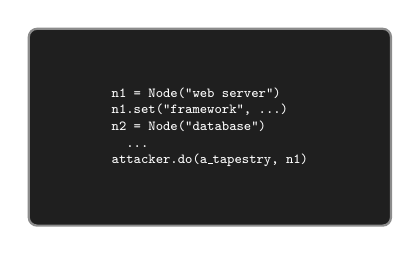
\begin{tikzpicture}
      \node[draw=black!45, thick, rounded corners=3pt, fill=black!88,
            text=white, font=\ttfamily\tiny, align=left,
            inner sep=3mm, minimum width=4.6cm, minimum height=2.5cm]
      {n1 = Node("web server")\\
       n1.set("framework", ...)\\
       n2 = Node("database")\\
       \ \ ...\\
       attacker.do(a\_tapestry, n1)};
    \end{tikzpicture}\\[3mm]
    {\footnotesize\color{inkGrey}proof of concept\\ a \emph{subset} of TIM}
  \end{column}
  \begin{column}{0.06\textwidth}
    \centering
    
\begin{tikzpicture}
      \draw[-{Stealth[length=5mm,width=4mm]}, line width=2.5pt, atkRed]
            (0,0) -- (0.9,0);
    \end{tikzpicture}
  \end{column}
  \begin{column}{0.58\textwidth}
    \centering
    \fbox{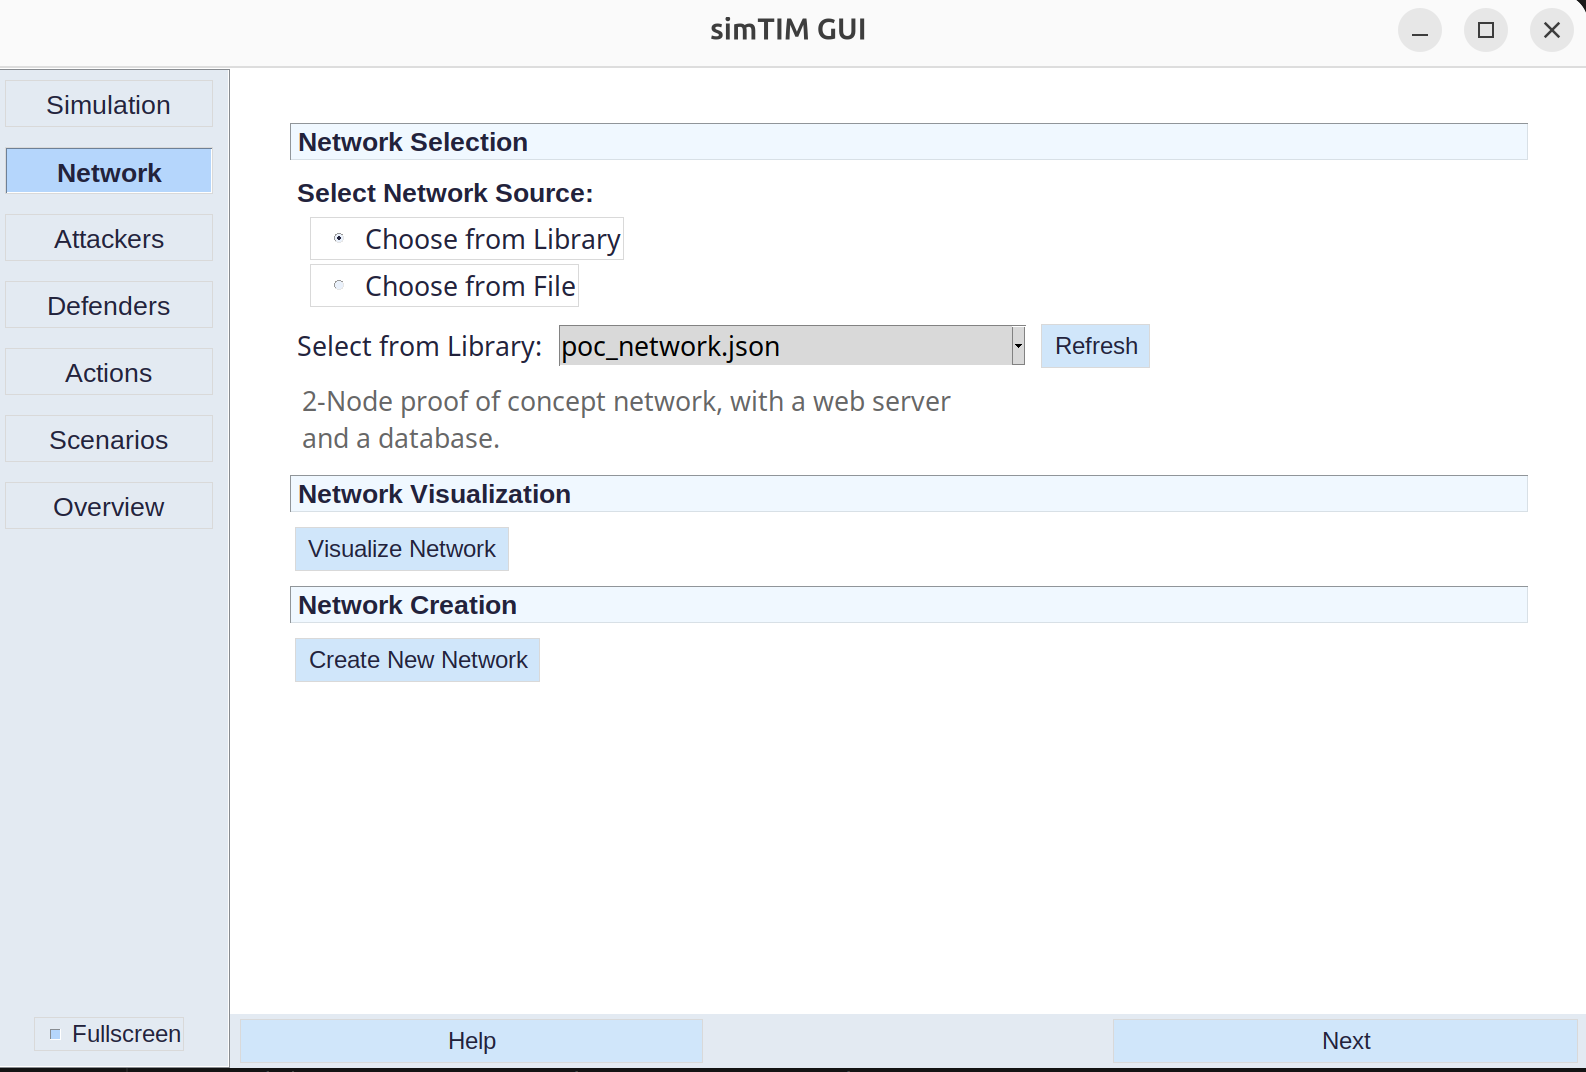
\includegraphics[width=\linewidth]{simTIM_GUI.png}}\\[2mm]
    {\footnotesize
     \textcolor{atkRed}{$\blacktriangleright$} graphical interface \quad
     \textcolor{atkRed}{$\blacktriangleright$} configurable simulations\\
     \textcolor{atkRed}{$\blacktriangleright$} Monte Carlo runs \quad
     \textcolor{atkRed}{$\blacktriangleright$} visualisation}
  \end{column}
\end{columns}
\vfill
\note{%
\textbf{2:30--3:00.} Respectful --- the proof of concept did its job.\\
The original TIM paper came with a small proof-of-concept program, implementing
only a subset of TIM's capabilities.\\
This is where simTIM comes in. simTIM aims to be a full implementation of the
TIM meta-model: a user-friendly graphical interface, easily configurable
simulations, Monte Carlo runs, and visualisation along the way.\\
Then: ``instead of talking about it, let me show you.''%
}
\end{frame}

% ===========================================================================
\begin{frame}[standout]
  Demonstration
  \note{%
  \textbf{3:00--8:15. Narrate the walkthrough. Do not improvise.}\\
  \emph{Simulation tab} --- one week, preset. Stochastic, so not one run but
  many; three runs for the demo. Detection bias set to \emph{early}: an action
  is most likely to be detected just after it starts.\\
  \emph{Network tab} --- networks are JSON, saved and loaded from file. Show the
  network creation tool.\\
  \emph{Attacker} --- how many, which strategy, capacity (how many actions at
  once), starting budget. Escalation: gain high privilege, then move laterally.
  Capacity infinite.\\
  \emph{Defender} --- budget and strategy too, but capacity is limited.\\
  \emph{Actions} --- defence capabilities; attackers can be given zero-days to
  better reflect reality. Mapped to MITRE ATT\&CK and D3FEND.\\
  \emph{Scenario comparison} --- compare parameters against each other. Here:
  different defence durations.\\
  \emph{Overview}, then run.\\
  \emph{Results} --- dashboard; event histories per run and per actor; economic
  timeline (damage, gain, cost); access timeline; then \textbf{attack path ---
  press play} and let it run.\\
  \emph{Statistical analysis} --- the scenario comparison. \textbf{Use the
  verified number: two hours instead of eight is less than half the damage, and
  it flattens out past about eight hours.} Same network, same actors, same
  success probabilities --- only time changed.\\
  If the video fails: backup slide has the dashboard screenshot.%
  }
\end{frame}

% ===========================================================================
\begin{frame}[plain]{Open source and extensible}
\vfill
\begin{columns}[c,onlytextwidth]
  \begin{column}{0.34\textwidth}
    \centering
    \qrcode[height=3.4cm]{https://github.com/noahbehrisch/simTIM}\\[3mm]
    {\footnotesize\ttfamily github.com/noahbehrisch/simTIM}\\[1mm]
    {\scriptsize\color{inkGrey}Apache 2.0 \quad$\cdot$\quad
     \textcolor{atkRed}{actively developed}}
  \end{column}
  \begin{column}{0.62\textwidth}
    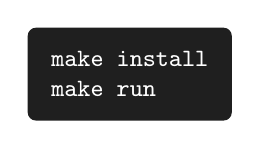
\begin{tikzpicture}
      \node[font=\ttfamily\small, text=white, fill=black!88, rounded corners=3pt,
            inner sep=3mm, anchor=north west, align=left]
            at (0,0) {make install\\make run};
    \end{tikzpicture}

    \vspace{5mm}
    {\large Four places to plug in:}\\[2mm]
    \begin{tabular}{@{}ll@{}}
      \textcolor{atkRed}{$\blacktriangleright$} & networks \quad{\scriptsize\color{inkGrey}(JSON)}\\[1mm]
      \textcolor{atkRed}{$\blacktriangleright$} & actions \quad{\scriptsize\color{inkGrey}(JSON)}\\[1mm]
      \textcolor{atkRed}{$\blacktriangleright$} & \textbf{strategies} \quad{\scriptsize\color{inkGrey}(one class)}\\[1mm]
      \textcolor{atkRed}{$\blacktriangleright$} & detection engines \quad{\scriptsize\color{inkGrey}(one class)}\\
    \end{tabular}
  \end{column}
\end{columns}
\vfill
\note{%
\textbf{8:15--8:50. Last slide --- leave the QR code up during questions.}\\
Apache 2.0, on GitHub, two commands to run it. And say plainly that it is still
under active development --- that is an invitation, not a disclaimer.\\
Apache 2.0, on GitHub, two commands to run it.\\
Four places to plug in. Be honest about the third one: our strategies today are
deliberately simple --- escalation, greedy, reactive, proactive. Real adversaries
are adaptive and coordinated. We built the arena; better players are exactly
what we hope the community brings.\\
Bring your own network, your own actions, your own strategy. Issues and pull
requests welcome.%
}
\end{frame}

\end{document}
